\documentclass{beamer}

\usepackage{beamerthemesplit}
\usepackage{verbatim}

\usetheme{Pittsburgh}
%\usecolortheme{seagull}
%\usecolortheme{seahorse}
\usecolortheme{beaver}

\usefonttheme{serif}

\newcommand{\snT}{$(S/N)_{\textrm{size}}$}
%\newcommand{\snT}{$\left( \frac{S}{N}\right)_{\textrm{size}}$}
\newcommand{\snflux}{$(S/N)_{\textrm{flux}}$}
%\newcommand{\snflux}{$\left( \frac{S}{N}\right)_{\textrm{flux}}$}

\title{Shear Estimation}
\author{Erin Sheldon}
\institute{Brookhaven National Laboratory}

% http://texblog.net/latex-archive/plaintex/beamer-footline-frame-number/
% to add the page (frame ) number and not screw up the bottom line
% works for split themes?
\expandafter\def\expandafter\insertshorttitle\expandafter{%
      \insertshorttitle\hfill%
        \insertframenumber\,/\,\inserttotalframenumber}


\begin{document}

\frame{\titlepage}

\%section{Introduction}

\frame
{
    \frametitle{Abell 370, HST}
    \includegraphics[width=\textwidth]{abell370_hst_med.jpg}
}
\frame
{
    \frametitle{Lensing Geometry and Deflection}
    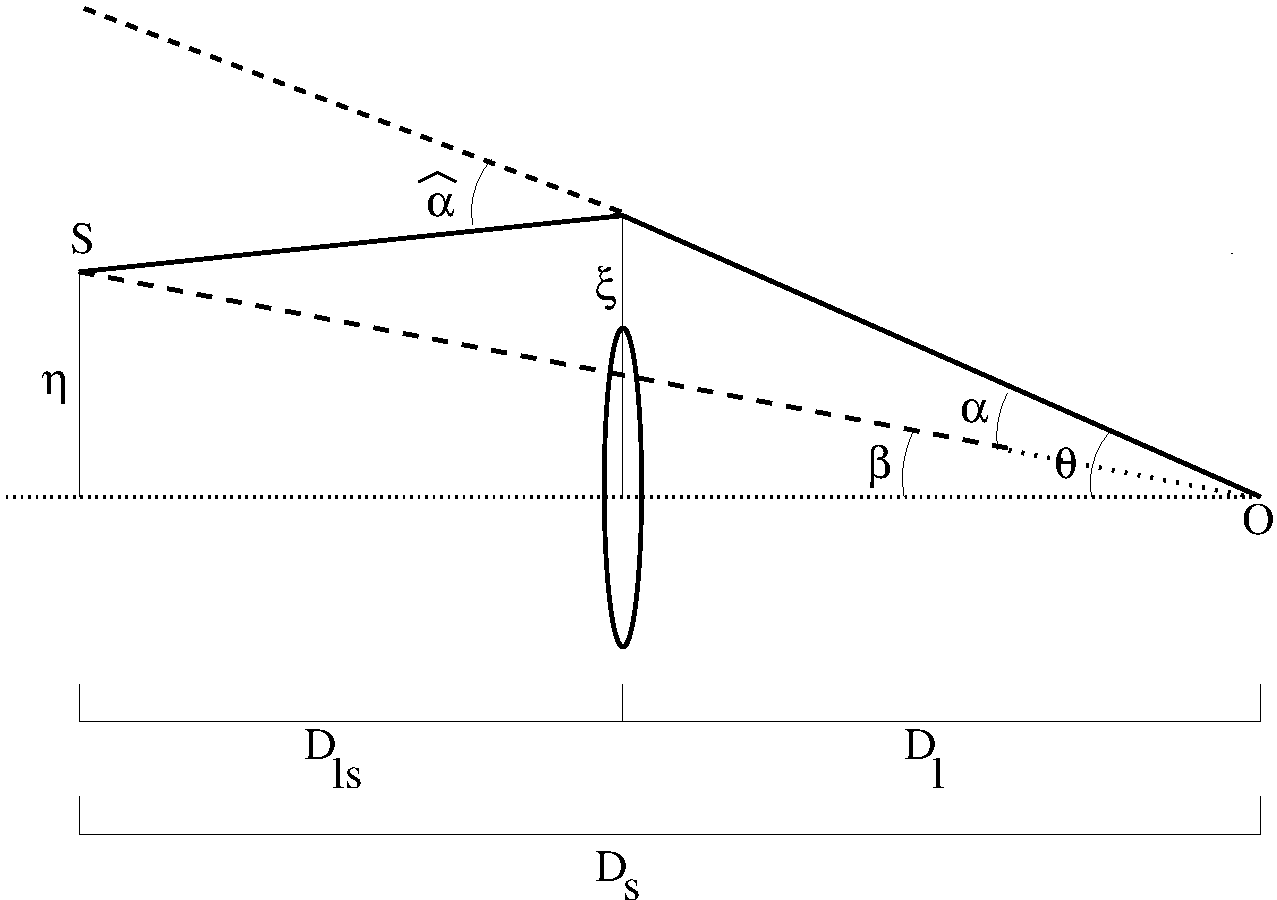
\includegraphics[width=\textwidth]{lens_geometry.pdf}
}

\frame
{
    \frametitle{Shear Illustration}
    \includegraphics[width=\textwidth]{shear-illustration.jpg}
}



\frame
{

    \frametitle{Gravitational Shear}

    \fontsize{10}{0.8\baselineskip}

    \begin{columns}

        \begin{column}{0.5\textwidth}

            \begin{itemize}
                \item The path of light appears curved as it passes massive objects
                \item The ``deflection'' can differ across the face of an extended source galaxy, causing distortion.
                \item Shear distorts the image; we say it's ``shape'' is altered.
                \item For small shears, a circle becomes a pure ellipse.
                \item Shearing produces correlations in the shapes of galaxies across the sky.
                    Shape correlations are closely related to mass density
                    correlations.

            \end{itemize}
        \end{column}
        \begin{column}{0.5\textwidth}
            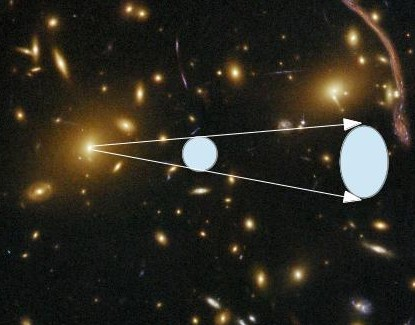
\includegraphics[width=\textwidth]{shear-illustration-crop.jpg}
            \newline
            \begin{center}
                {\small Note galaxies aren't round!  ``Shape noise''}
            \end{center}
        \end{column}
    \end{columns}
}

\frame
{
    \frametitle{Shear}
    \fontsize{10}{0.8\baselineskip}

    \begin{columns}
        \begin{column}{0.5\textwidth}
            \begin{itemize}

                \item The correlations in the shear/matter field hold a lot of
                    information about the {\bf Dark Matter} distribution.  The Cold Dark
                    Matter theory predicts these correlations.

                \item Shear depends on the distances to the lens and source. The
                    distance dependence encodes the expansion rate of the universe and
                    thus {\bf Dark Energy}.

                \item To meet goals of current surveys we want to measure shear to
                    about 0.3-0.4\% accuracy (e.g.  Dark Energy Survey).  LSST about
                    a factor of five better.

            \end{itemize}
        \end{column}

        \begin{column}{0.5\textwidth}
            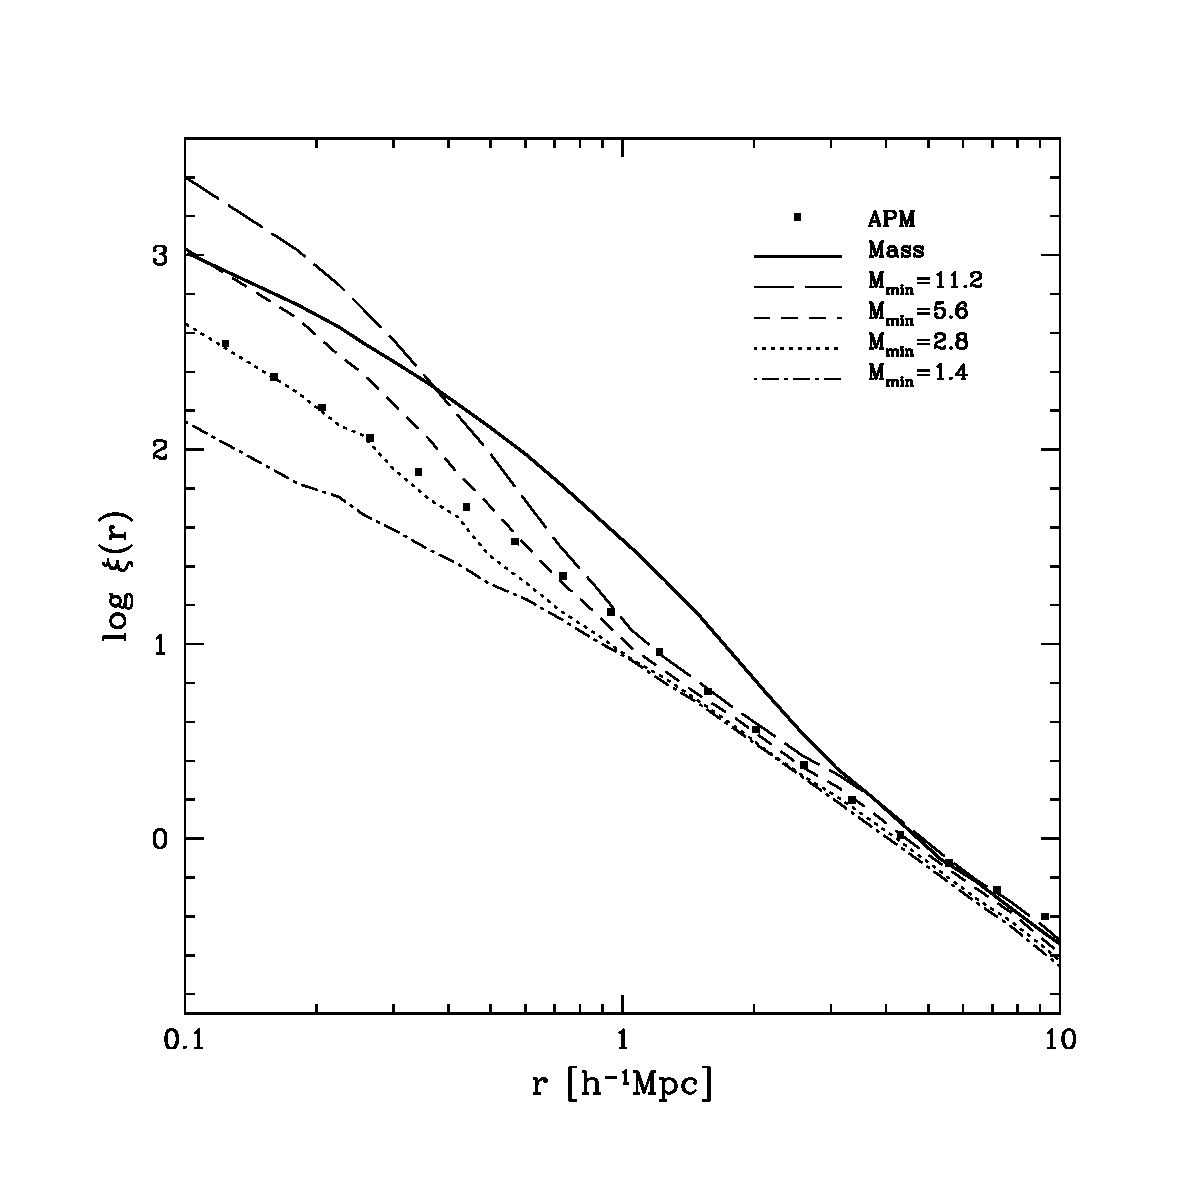
\includegraphics[width=\textwidth]{berlind-weinberg-f3.pdf}
            \newline
            \begin{center}
                {\tiny Berlind \& Weinberg 2002}
            \end{center}
        \end{column}
    \end{columns}
}



\frame
{
    \frametitle{Measuring Shear}

    \begin{itemize}
        \item For a perfect detector with no noise, just measure
            the second moments and look for the correlations.
        \item ... but the atmosphere, telescope, and instrument smear
            the image: the Point Spread Function (PSF).
        \item Convolution just adds to the moments, so we just need to
            subtract off the PSF moments!

        \item ... but there is noise, so error in moments blows up (among other
            difficulties).

    \end{itemize}
}

\frame
{
    \frametitle{PSF and Noise}
    
    \begin{itemize}

        \item One can use a weight function to suppress the noise, but then one
            must derive how that measurement responds to smearing by the PSF
            and shearing (e.g. Kaiser, Squires, \& Broadhurst, Bernstein \& Jarvis, Melchior,
                    Bernstein \& Armstrong).  Working in Fourier space can help
            with the deconvolution (Bernstein).

        \item Alternatively, one can forward-model the problem: fit a model that is
            convolved with an estimate of the PSF.  Limited by how well one can
            model the galaxy and PSF (e.g. Miller et al., Bernstein \& Armstrong, many
            others).

        \item These methods can be made to work well, as long as the $S/N$ is
            still pretty high, say 50 or higher.

    \end{itemize}
}

\frame
{
    \frametitle{Noise}

    \begin{itemize}
        \item When the $S/N$ is low, these techniques break down.

        \item Non-linear fitting in the presence of noise is biased, both the
            maximum likelihood and expectation value: using the mean shape
            won't work (Hirata, Refregier, etc).   Results in a {\bf
            calibration} error.

        \item This is generally known in statistics, but not yet solved
            for our particular problem. Badly aggravated by the PSF ``deconvolution''.
        \item The noise also causes problems for moment based methods.
    \end{itemize}
}

\frame
{
    \frametitle{Maximum Likelihood}

    \begin{center}
    \includegraphics[width=0.7\textwidth]{{gmix-fit-gg05r01-yr-0.005-0.005-diff}.pdf}
\end{center}

}

%\section{Bayesian Methods}

\frame
{
    \frametitle{Miller et al. 2007}

    \begin{itemize}

        \item Miller et al. 2007 (LENSFIT): Use priors on the parameters and
            explore a constrained posterior surface (Prior $\times$
            Likelihood).

        \item Attempt to derive how the shear estimate (the shape) affected by
            the noise and prior using integrals over the posterior surface and
            first order approximation in shear.  Called the {\bf response}.

        \item The posterior surface of the shape for a single galaxy is
            complex.  The space is bounded, the surface is necessarily
            asymmetric and depends on galaxy properties and noise.

        \item No rigorous expression is given for the mean shear of a
            population given these ellipticity responses.  Choose to simply
            average them.

        \item Miller et al. 2013 find large biases in simulations, of
            order 10\% at \snflux$ \sim 10$.
        
    \end{itemize}
}

\frame
{
    \frametitle{LENSFIT Tests}

    \begin{columns}
        
        \begin{column}{0.5\textwidth}
            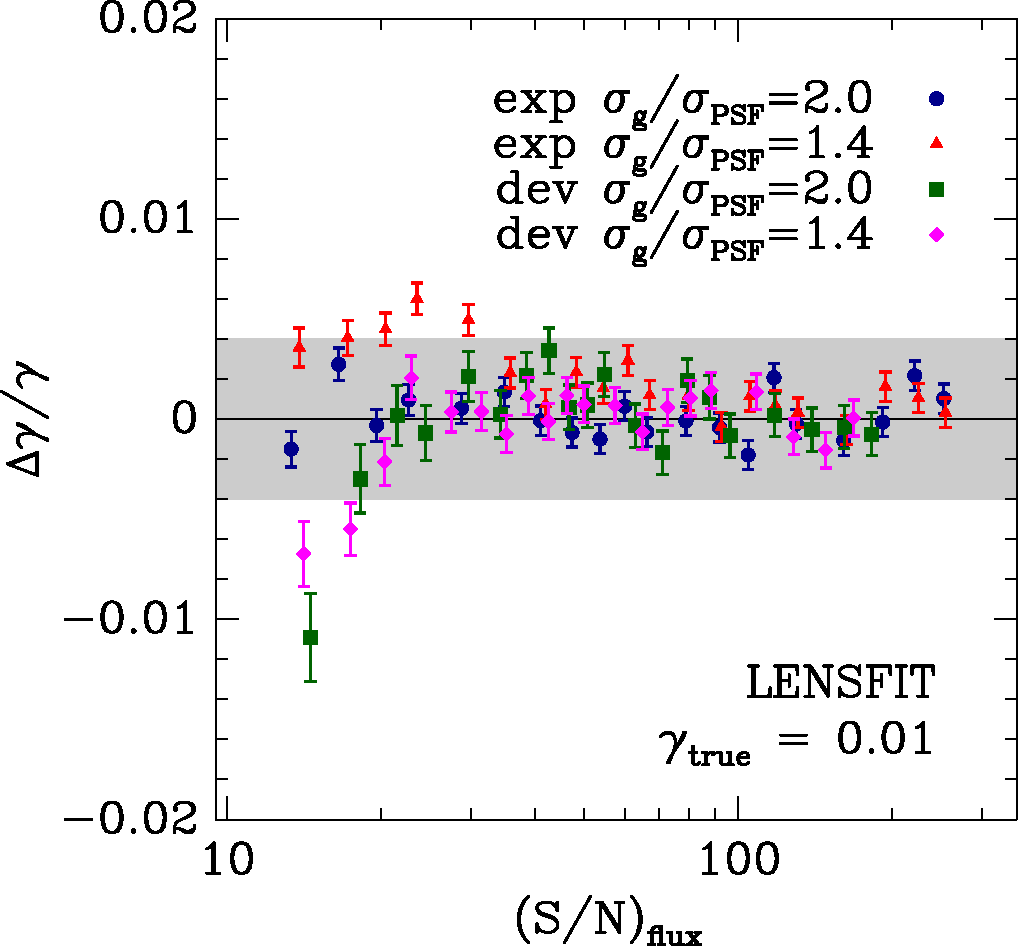
\includegraphics[width=\textwidth]{cbafit-geg07-geg08-deg03-deg05-lensfit-flux-s2n.pdf}
        \end{column}

        \begin{column}{0.5\textwidth}
            \includegraphics[width=\textwidth]{cbafit-geg07-geg08-deg03-deg05-lensfit-T-s2n.pdf}
        \end{column}
    \end{columns}

    \fontsize{9}{0.8\baselineskip}
    \begin{itemize}
        \item I did my own tests of LENSFIT with strong structural priors (30\% lognormal
            on flux, 15\% on size (that was a bug...) ).

        \item Very fast code using gaussian mixtures to approximate galaxies.  Fast
            analytic convolutions.

        \item Bias vs \snT\ has more universal form than vs \snflux.
    \end{itemize}

}

\begin{comment}
\frame
{
    \frametitle{Shear of the Light Distribution}

    \begin{itemize}

        \item Stack the light around peaks in images.

        \item Assume the shear is constant over the patch of interest.

        \item This two-dimensioinal correlation function of the light is
            sheared just as galaxy images are.  Don't need to de-blend.  Not
            fully explored (ES).

    \end{itemize}
}
\end{comment}

\frame
{
    \frametitle{Bernstein \& Armstrong 2013}

    \begin{itemize}

        \item Shape is not shear.
        \item While the posterior surface for the {\it shape} of single galaxy
            is complex, the posterior surface for the {\it mean shear} of an
            ensemble must approach a Gaussian according to the central limit
            theorem.  This is both useful and actually true!

         \item Assuming Gaussianity, weak shear, and knowledge of underlying
             distribution of shapes for the ensemble (the prior), one can
             derive an unbiased estimator for the mean shear of the ensemble.

         \item You lose nothing: in the limit of weak shear, you need
             to use an ensemble statistic anyway.  The ``shape noise'',
             intrinsic variance in shapes of galaxies, dominates over
             the signal.

        \item This is a good idea, but needed an implementation, so I worked it
            into my existing code.
         
    \end{itemize}

}

\frame
{
    \frametitle{BA13 Tests}

    \begin{columns}
        
        \begin{column}{0.5\textwidth}
            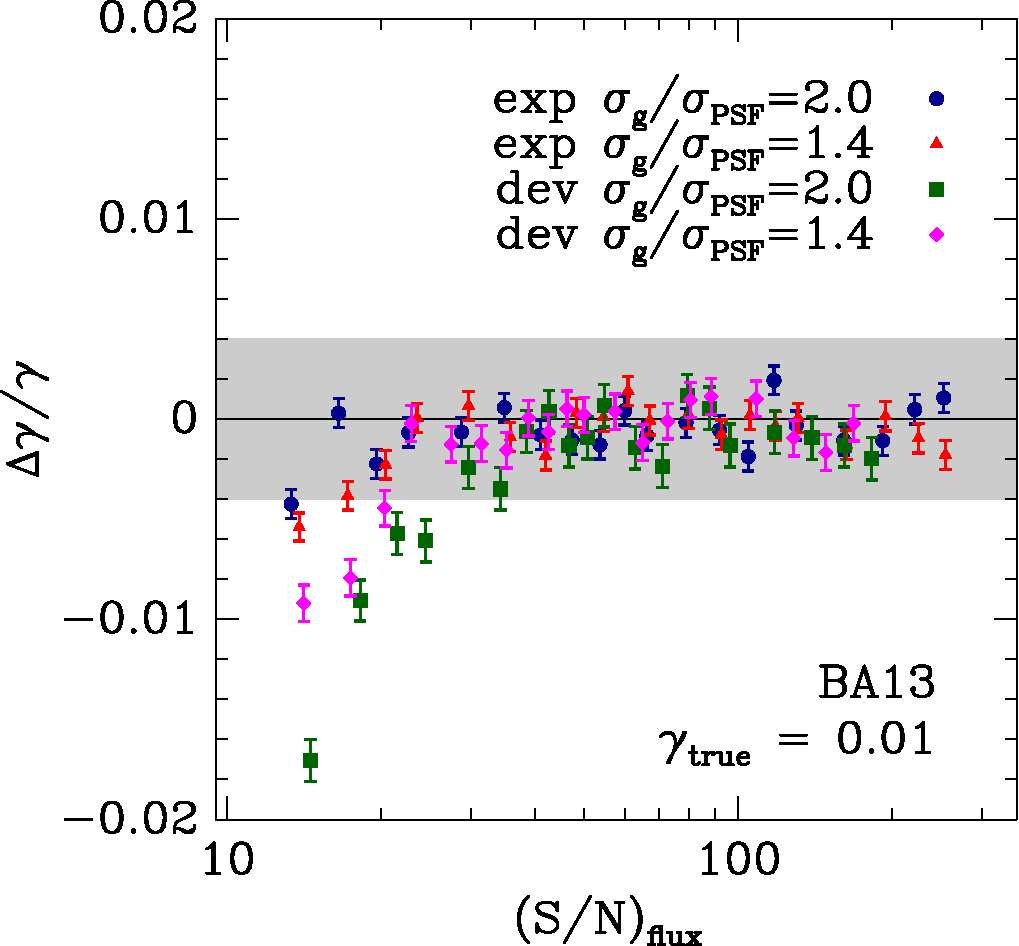
\includegraphics[width=\textwidth]{cbafit-geg07-geg08-deg03-deg05-ba13-flux-s2n.pdf}
        \end{column}

        \begin{column}{0.5\textwidth}
            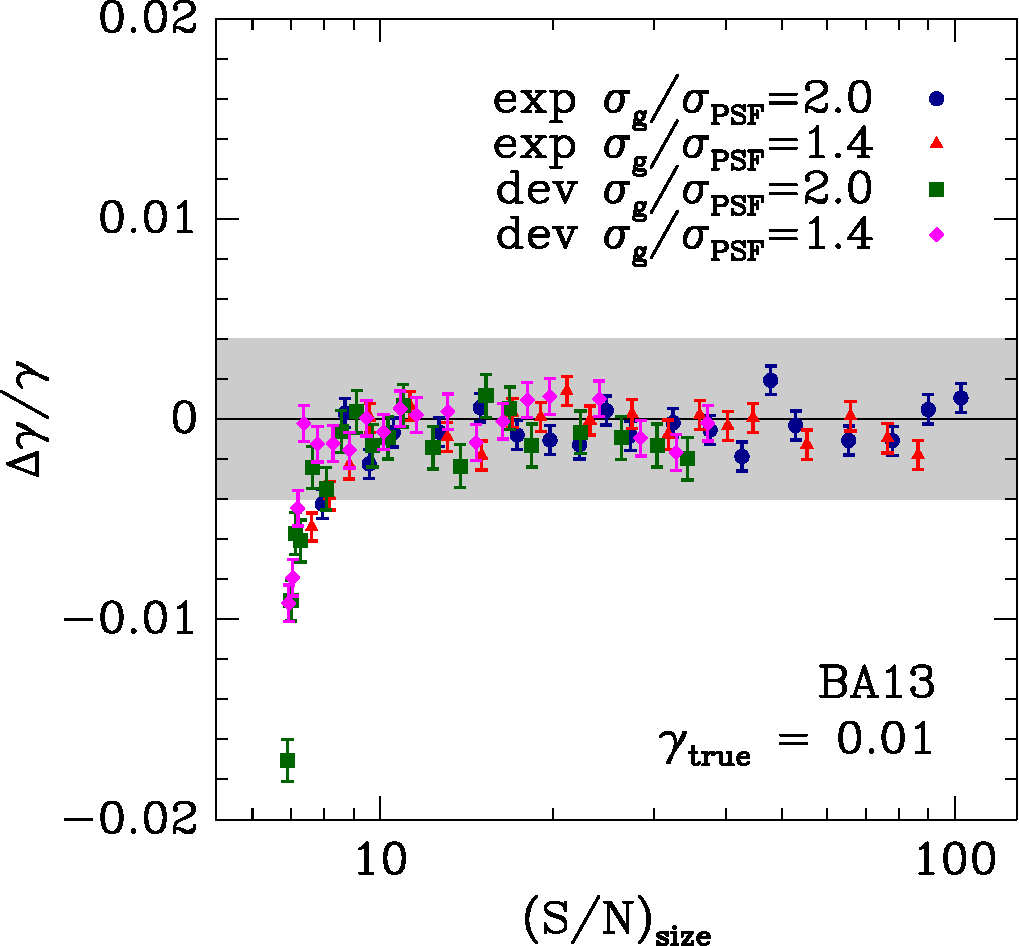
\includegraphics[width=\textwidth]{cbafit-geg07-geg08-deg03-deg05-ba13-T-s2n.pdf}
        \end{column}
    \end{columns}

    \begin{itemize}
        \item Assuming we can find the right model.
        \item Sufficient accuracy for DES at \snT$ > 10$.
    \end{itemize}
}

%\section{Summary}

\frame
{
    
    \frametitle{Bernstein \& Armstrong 2013 Tests}

    \begin{itemize}
        \item Can push to lower \snT\ than LENSFIT.

        \item Bias varies with \snT\ in a simpler way than LENSFIT.
        \item Bias vs \snT\ even more universal. Sufficient accuracy for DES at \snT$ > 10$.

       

    \end{itemize}
}

\frame
{
    \frametitle{Limitations}
    \begin{itemize}

        \item I'm assuming I can find the right model.  Not true in real data.
            Should be OK for DES (Kacprzak et al. 2013) but not LSST.

        \item TODO: 
            
            \begin{itemize}

                \item Explore more realistic intrinsic distributions in
                    structural parameters (size, flux).  E.g. for a bin in {\it
                    measured} flux, what are the {\it true} distributions in
                    size and flux?  Use Cosmos.

                \item Why is there bias at all?  Is it the likelhood sampling method?

                \item Bernstein \& Armstrong propose a model-independent
                    technique using moments in Fourier space, but not yet
                    implemented.  Gary and Bob plan to do it.  Student at Stony
                    Brooke as well (Madhavacheril).

            \end{itemize}

    \end{itemize}
}
\frame
{
    \frametitle{Summary}

    \begin{itemize}

        \item Shear estimation is difficult in the presence of noise.

        \item Modern techniques can work well enough for current surveys.

        \item For future experiments such as LSST we need a model-independent
            approach.

    \end{itemize}
}

\end{document}
